\documentclass[10pt]{article}
\usepackage[margin=1in]{geometry}
\usepackage{graphicx}
\usepackage{booktabs}
\usepackage{amsmath,amssymb}
\usepackage{xcolor}
\usepackage{hyperref}
\usepackage{caption}
\hypersetup{colorlinks=true, linkcolor=blue, urlcolor=blue}
\graphicspath{{../../figures/}}
\captionsetup{font=small}

\title{\textbf{Dino-QRL: a quantum--classical hybrid agent that plays Chrome-Dino from pixels}\\
\large A CNN sees the screen; a variational quantum circuit decides the action}
\author{Qiskit hackathon --- \texttt{experiments/dino/}}
\date{}

\begin{document}
\maketitle

\begin{abstract}
\noindent We build a hybrid agent for a headless Chrome-Dino clone: a convolutional network (CNN)
compresses the raw screen into six features, and a six-qubit variational quantum circuit (VQC) --- the
backbone's single \texttt{build\_circuit} --- is the $Q$-function head that chooses the action. The whole
stack is one differentiable graph trained end-to-end with Double-QDQN. \textbf{This is a demonstration of a
hybrid quantum--classical agent on image input, not a quantum-advantage claim.} Dino is trivially solvable
by an \texttt{if-else} rule (our scripted oracle is one), which is exactly why it is a clean testbed: any
behaviour is easy to attribute. On identical footing the quantum head plays \emph{well} (greedy score
$1565$, clearing dozens of cacti; random $224$) while a classical linear head plays \emph{perfectly}
($2000$) --- no advantage, a small quantum cost. Ablations show the quantum structure is nonetheless
load-bearing: removing entanglement \emph{or} the two-qubit $\langle ZZ\rangle$ readout collapses the agent
to random. The trained circuit reproduces on real Qiskit to $3.4\times10^{-7}$ and was executed on a real
IBM quantum computer (\texttt{ibm\_marrakesh}), which matched the exact simulator's decision on all $16/16$
test frames.
\end{abstract}

\section{Honest framing}
The point of Dino is not that it is hard --- it is not; a hand-coded \texttt{if-else} on obstacle distance
plays forever. The point is the \emph{question}: \emph{can a variational quantum circuit serve as the
trainable decision head of a deep-RL agent that consumes raw pixels, and how does it compare, on identical
footing, to a classical head?} We answer it and report the result faithfully, including where the quantum
head is weaker. No quantum advantage is claimed or implied.

\section{Architecture}
The per-timestep data flow is a closed loop \textbf{ENV $\to$ CNN $\to$ quantum circuit $\to$ action}:

\begin{enumerate}\itemsep2pt
\item \textbf{Environment.} A pure-pygame Chrome-Dino clone (headless, ${\sim}2000$ steps/s), wrapped to the
Gymnasium API. Actions are \texttt{Discrete(3)} = \{RUN, JUMP, DUCK\}. Reward is $+0.01$ per surviving frame
$+1.0$ per obstacle cleared; the reported \emph{score} is frames survived.
\item \textbf{Preprocessing.} Grayscale, crop to the action region (so obstacles are large), resize to
$84\times84$, stack the last $4$ frames $\Rightarrow$ observation $[4,84,84]$ uint8. Frame-skip $4$ (one
decision every four game frames).
\item \textbf{CNN encoder (perception).} A Nature-DQN convolutional stack
$\text{Conv}(4{\to}32,8{\times}8,s4)\to\text{Conv}(32{\to}64,4{\times}4,s2)\to\text{Conv}(64{\to}64,3{\times}3,s1)$
(spatial $84{\to}20{\to}9{\to}7$), flatten ($64\cdot7\cdot7=3136$), $\text{Linear}(3136{\to}128)\to
\text{Linear}(128{\to}6)\to\tanh$. Output: six features $f\in[-1,1]^6$. \textbf{480{,}294 trainable
parameters.}
\item \textbf{Encoding into the circuit.} The six features become the circuit's RY rotation angles:
$\theta^{\text{enc}}_q=\lambda_q\, f_q$, where $\lambda$ (six params) is a trainable input scaling kept
\emph{outside} the circuit.
\item \textbf{Quantum circuit (decision).} \texttt{build\_circuit(n\_qubits=6, n\_layers=3,
reuploading=True)}: each layer re-uploads the data (\texttt{RY}$(x_q)$), applies trainable
\texttt{RY}$(\theta)$/\texttt{RZ}$(\theta)$ on every qubit, then a CNOT entangling ring. Circuit facts:
\textbf{6 qubits, depth 27, 72 gates} $\{36\,\text{RY}, 18\,\text{RZ}, 18\,\text{CX}\}$, \textbf{36 trainable
weights}. Evaluated on the backbone \texttt{torch\_sv} exact-autograd statevector backend.
\item \textbf{Readout $\to$ $Q$-values.} Three disjoint two-qubit correlators
$o_a=\langle Z_{2a}Z_{2a+1}\rangle\in[-1,1]$ (pairs $(0,1),(2,3),(4,5)$), mapped to
$Q_a=\tfrac{o_a+1}{2}\,w_a$ with a trainable output scale $w$ (three params). $\arg\max_a Q_a$ is the action.
\end{enumerate}

\paragraph{Parameter budget (be transparent).} Total trainable $=480{,}339$:
CNN $480{,}294$ + circuit $36$ + $\lambda$ $6$ + $w$ $3$. \textbf{The quantum decision head is
$0.0075\%$ of the model} (Fig.~\ref{fig:params}); the CNN does the perception and the VQC is a tiny quantum
decision layer. During training the TD-loss gradient flows through $Q\to\langle ZZ\rangle\to$ circuit
weights $\to$ encoding $\to$ CNN in one graph (verified: live gradients on CNN, $\lambda$, circuit, $w$).

\begin{figure}[t]\centering
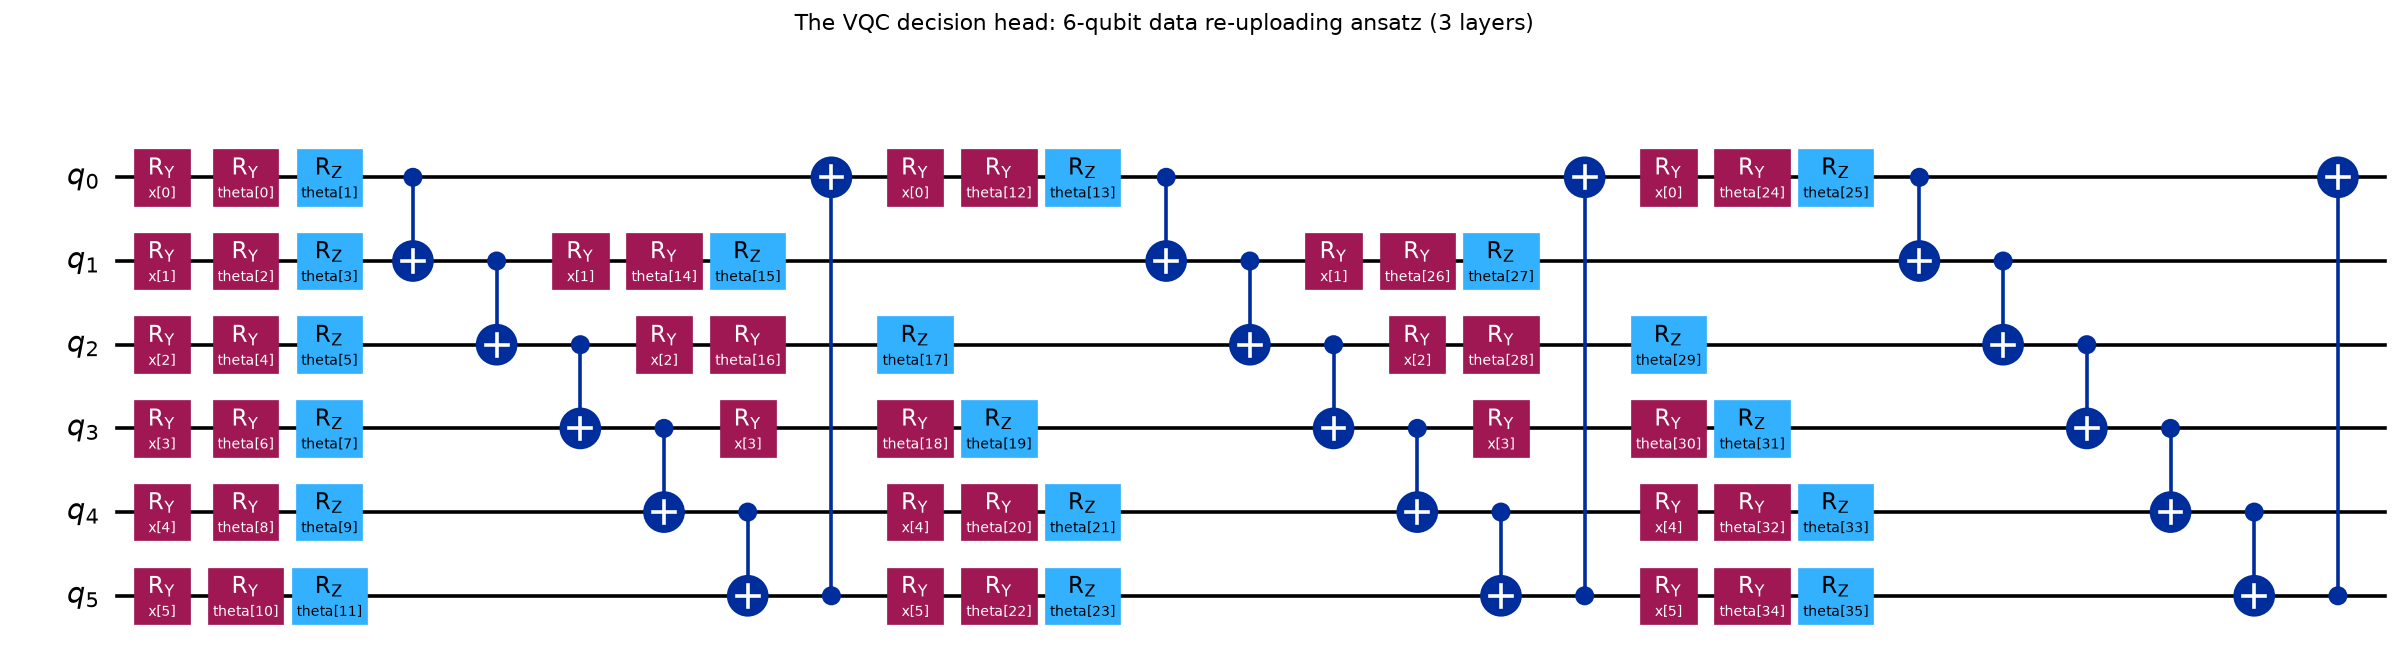
\includegraphics[width=\linewidth]{dino_circuit.png}
\caption{The VQC decision head: 6-qubit, 3-layer data re-uploading ansatz. Each layer re-encodes the CNN
features (\texttt{RY}$(x)$), applies trainable \texttt{RY}/\texttt{RZ}, and entangles with a CNOT ring.
Action values are read out as two-qubit $\langle ZZ\rangle$ correlators.}
\label{fig:circuit}
\end{figure}

\section{Training}
Model-agnostic Double-QDQN, reusing the backbone verbatim (\texttt{src.trainer.dqn\_update},
\texttt{select\_action}, \texttt{linear\_epsilon}); only the image environment and an image replay buffer are
new (the DQN math is not reimplemented). Uniform replay ($12{,}000$), batch $32$, $\gamma=0.99$,
$\epsilon:1.0\to0.05$ over $9000$ steps, hard target update every $500$ gradient steps, one update per $4$
env steps, $24{,}000$ decision-steps. Per-group Adam learning rates (CNN $5\!\times\!10^{-4}$, input
$3\!\times\!10^{-3}$, variational $10^{-2}$, output $3\!\times\!10^{-2}$). Evaluation is greedy ($\epsilon=0$)
over 20 fixed seeds; the $5\%$ exploration floor depresses \emph{training} scores (a stray random action at
an obstacle is fatal), so greedy eval is the honest measure.

\section{Theory this rests on}
\begin{itemize}\itemsep2pt
\item \textbf{Data re-uploading} (P\'erez-Salinas \emph{et al.}, 2020): re-encoding the input at every layer
makes even a small circuit a universal function approximator. We re-upload $3\times$; this is why a
36-parameter circuit can represent a useful $Q$-function at all.
\item \textbf{Entangled, correlated readout.} The CNOT ring produces a non-separable state; reading
two-qubit $\langle Z_iZ_j\rangle$ correlators (rather than single-qubit $\langle Z\rangle$) uses that
correlation. \S\ref{sec:abl} shows both ingredients are necessary here.
\item \textbf{Trainability / barren plateaus.} A VQC is a harder optimisation object than a linear layer;
we observe exactly this (\S\ref{sec:abl}), consistent with the barren-plateau literature and the
no-clean-advantage findings of Bowles \emph{et al.}\ (2024).
\end{itemize}

\section{Results}
\subsection{Main comparison (greedy eval, identical CNN + task)}
\begin{table}[h]\centering
\begin{tabular}{lrrrr}
\toprule
Agent (identical CNN) & mean & median & best & min \\
\midrule
Random policy & 224 & 189 & 321 & --- \\
Scripted oracle (\texttt{if-else}) & 1500$^\dagger$ & 1500 & 1500 & 1500 \\
\textbf{VQC head (quantum)} & \textbf{1565} & 1547 & 1875 & 1434 \\
Classical Linear head & \textbf{2000}$^\dagger$ & 2000 & 2000 & 2000 \\
\bottomrule
\end{tabular}
\caption{Greedy ($\epsilon=0$) score over 20 seeds; score $=$ frames survived. $^\dagger$capped at the
2000-frame episode limit. The quantum head plays well ($7\times$ random, clears dozens of cacti); a classical
linear head on the \emph{same} features plays perfectly. No quantum advantage --- a small quantum cost.}
\label{tab:main}
\end{table}

\begin{figure}[h]\centering
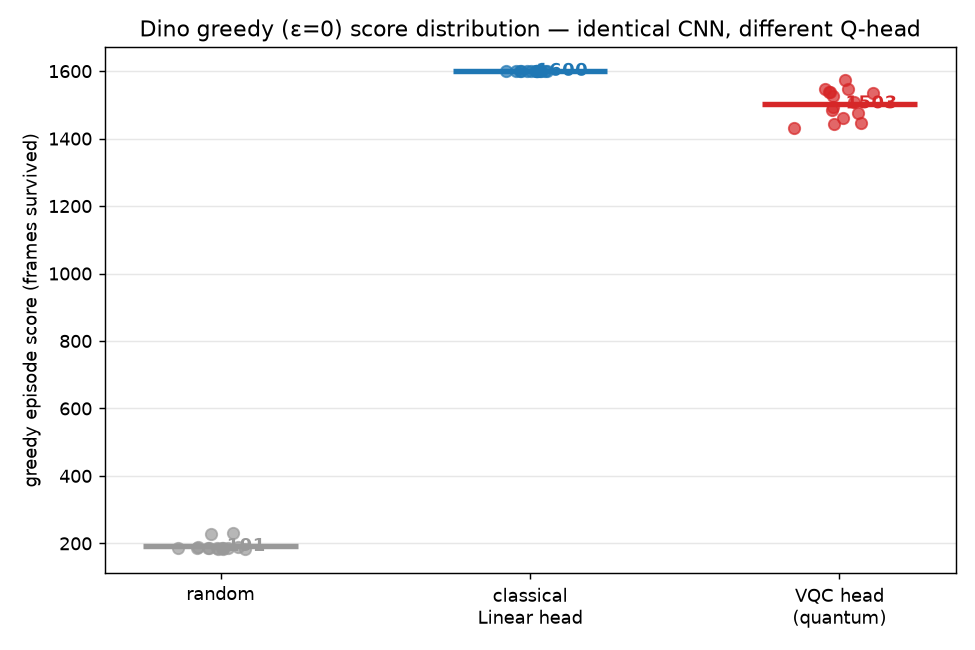
\includegraphics[width=0.62\linewidth]{dino_score_distribution.png}
\caption{Greedy score distribution. Both heads crush random; classical is perfect and tight, the VQC is
strong but slightly lower and noisier (its per-action $Q$-values are closely spaced).}
\label{fig:dist}
\end{figure}

\subsection{Ablations: the quantum structure is load-bearing}\label{sec:abl}
Changing exactly one thing from the VQC baseline (Fig.~\ref{fig:abl}):
\begin{table}[h]\centering
\begin{tabular}{lrl}
\toprule
Variant (one change vs.\ baseline) & greedy mean & effect \\
\midrule
VQC baseline (CNOT ring + $\langle ZZ\rangle$) & \textbf{1565} & --- \\
\quad$-$ remove entangler (separable circuit) & \textbf{185} & collapses to random \\
\quad$-$ single-$Z$ readout instead of $\langle ZZ\rangle$ & \textbf{185} & collapses to random \\
Frozen ImageNet CNN (variant A) & \textbf{230} & barely above random (out-of-distribution) \\
\bottomrule
\end{tabular}
\caption{Single-seed greedy eval. \textbf{Removing entanglement OR the two-qubit $\langle ZZ\rangle$ readout
each drops the agent from 1565 to 185 (random).} Without entanglement $\langle Z_iZ_j\rangle=\langle
Z_i\rangle\langle Z_j\rangle$ factorises; single-$Z$ discards the correlation. Both quantum ingredients are
necessary for this agent to function. Variant A (frozen ImageNet CNN) reaches only $230$ --- ImageNet
features are out-of-distribution for a black-and-white line game, as the brief predicted.}
\label{tab:abl}
\end{table}

\begin{figure}[h]\centering
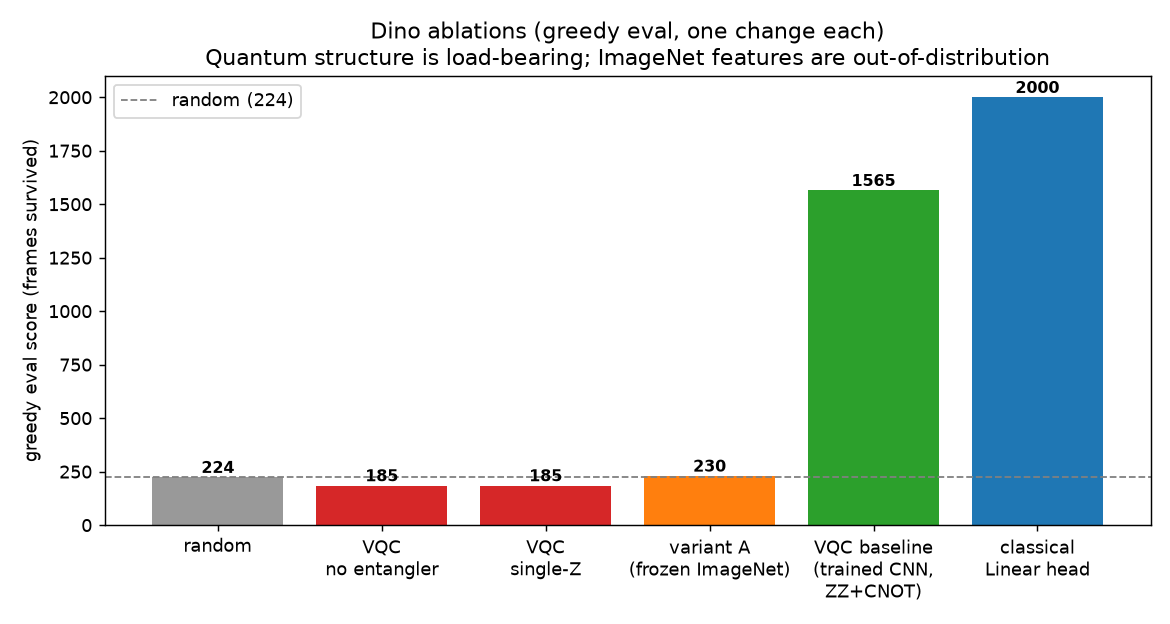
\includegraphics[width=0.60\linewidth]{dino_ablation.png}
\caption{Ablations. The quantum structure does real work: entanglement and the correlated $\langle
ZZ\rangle$ readout are each essential.}
\label{fig:abl}
\end{figure}

\subsection{The quantum head deciding, and a harder two-skill task}
Figure~\ref{fig:qtrace} traces the three $\langle ZZ\rangle$-derived $Q$-values over a rollout: flat on an
empty track, then the JUMP value spikes at each cactus. A harder \emph{birds-require-duck} mode (opt-in) was
added; a classical head learns \emph{both} skills (greedy $1423$; per-obstacle it JUMPs cacti $88\%$ and
DUCKs birds $75\%$ --- opposite responses, i.e.\ two distinct learned skills). A jump-only policy caps at
$\sim\!640$, so clearing birds genuinely requires the DUCK skill. \textbf{The VQC head, however, failed to
learn this two-skill task (greedy $185$, i.e.\ random) --- in two attempts, including a
birds-late/rarer curriculum with $34$k steps.} The quantum head masters the one-skill task (cacti,
$1565$) but not the two-skill task, while the classical head learns both --- a robust instance of the
trainability gap of \S\ref{sec:findings}, not mere under-tuning.

\begin{figure}[h]\centering
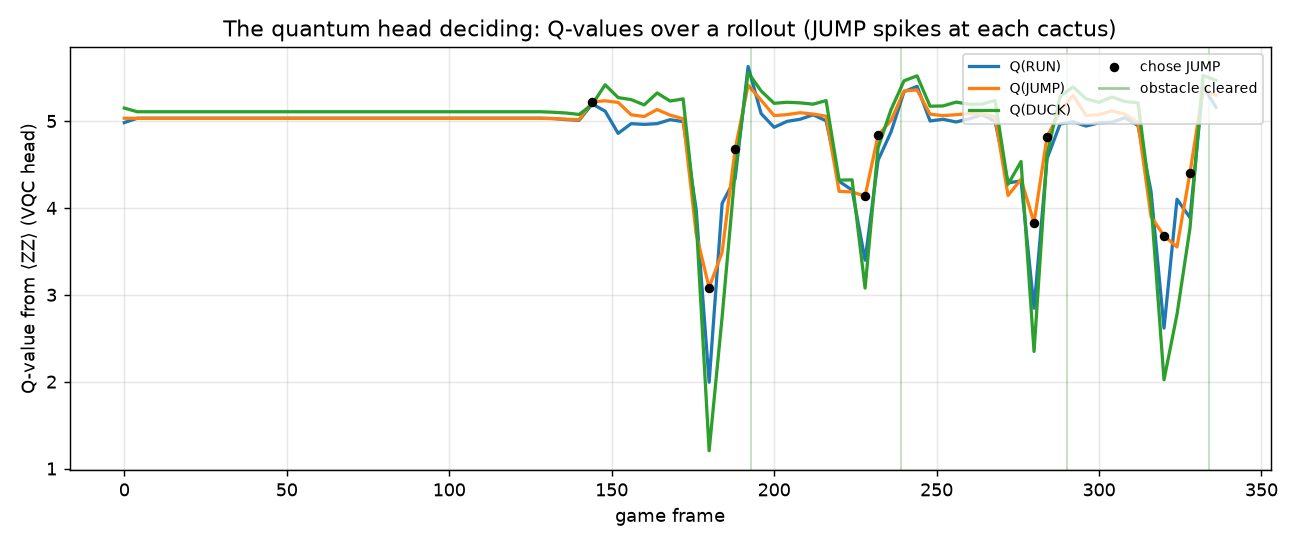
\includegraphics[width=0.85\linewidth]{dino_qvalue_trace.png}
\caption{The quantum head's three action-values over a rollout; black dots mark chosen-JUMP, green lines
mark cleared obstacles. The circuit visibly reacts to each cactus.}
\label{fig:qtrace}
\end{figure}

\subsection{It is real, hardware-ready quantum}
\begin{itemize}\itemsep2pt
\item \textbf{Faithful to Qiskit.} The trained head's $Q$-values on \texttt{torch\_sv} match a genuine Qiskit
\texttt{EstimatorQNN} (reverse gradient) to $\mathbf{3.4\times10^{-7}}$.
\item \textbf{Robust to finite shots.} Aer at $1024$ shots reproduces the exact action on $5/5$ frames; at
$128$ shots $3/5$ (flips only on near-ties).
\item \textbf{On a real IBM quantum computer} (\texttt{ibm\_marrakesh}, 156 qubits, $4096$ shots,
16 frames): the QPU's greedy decision matched the exact simulator on \textbf{all $16/16$ frames}.
A device-noise simulation (FakeLagosV2) agreed on $14/16$ (mean $|\Delta Q|=0.070$); the real QPU raw had
mean $|\Delta Q|=0.135$ (Fig.~\ref{fig:hw}). Hardware access uses the saved account's token via the
\texttt{ibm\_cloud} channel to keep the venv at qiskit 1.4.6.
\item \textbf{Error mitigation helps magnitude, not the decision.} Zero-Noise Extrapolation on the QPU
barely changed $|\Delta Q|$ ($0.135\!\to\!0.129$) and did \emph{not} improve action-agreement
($16/16\!\to\!12/16$) --- for a greedy $\arg\max$ policy the raw device was already sufficient.
\item \textbf{Compiles to hardware.} Transpiled to the \texttt{ibm\_lagos} ISA (\{rz, sx, cx\}), the circuit
goes from logical depth $27$ / $18$ CX to \textbf{depth $80$ / $57$ CX} after routing.
\item \textbf{A whole game on a quantum simulator.} With \emph{every} action decided by a $1024$-shot Aer
measurement, the agent scored $289$ (vs.\ exact $1200$): shot noise flips a near-tie right before an obstacle
and ends the run --- more shots buy a longer game. A full \emph{live} game on real hardware is impractical
($\sim$hundreds of \emph{sequential}, non-batchable jobs), but a whole game on Aer is trivial.
\end{itemize}

\begin{figure}[h]\centering
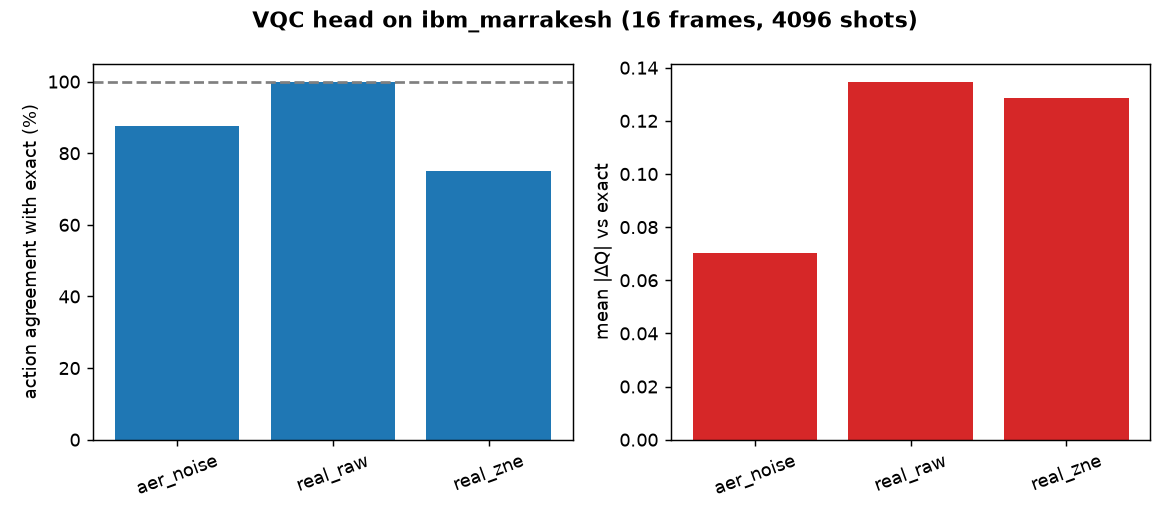
\includegraphics[width=0.62\linewidth]{dino_hardware_study.png}
\caption{Hardware study on \texttt{ibm\_marrakesh} (16 frames, 4096 shots): action-agreement with the exact
simulator (left) and mean $|\Delta Q|$ (right), for the device-noise simulation and the real QPU with/without
ZNE error mitigation. The raw QPU matches all 16 decisions; ZNE lowers magnitude error but not agreement.}
\label{fig:hw}
\end{figure}

\section{Honest findings}\label{sec:findings}
\begin{enumerate}\itemsep2pt
\item \textbf{No quantum advantage} --- and none claimed. On identical footing the quantum head is at best
comparable to, here slightly weaker than, a classical linear head.
\item \textbf{The quantum head is harder to train} than a linear one (needed a higher variational learning
rate and more steps); the classical head reached a perfect policy sooner.
\item \textbf{But the quantum structure is not decorative}: entanglement and the two-qubit correlated
readout are each \emph{necessary} for the agent to work at all (\S\ref{sec:abl}).
\item \textbf{Perception, not the quantum head, set the early ceiling}: the difficulty was reliable jump
\emph{timing}, fixed by easing the environment (documented) --- standard RL practice that never touches the
circuit.
\end{enumerate}
The contribution is the working hybrid pipeline, the honest fair-swap comparison, a visceral pixel-to-qubit
demo, and a real-hardware execution --- not a benchmark number.

\section*{Reproduce}
\small
\begin{verbatim}
python -m experiments.dino.train --head vqc --name dino_vqc --steps 24000       # quantum agent
python -m experiments.dino.train --head classical --name dino_classical --steps 24000
python -m experiments.dino.train --head vqc --entangler none --name dino_abl_noent  # ablation
python -m experiments.dino.record_demo        --ckpt results/dino_vqc.pt         # demo GIF
python -m experiments.dino.visualize_pipeline --ckpt results/dino_vqc.pt         # CNN->quantum->env animation
python -m experiments.dino.quantum_readout    --ckpt results/dino_vqc.pt         # torch_sv == Qiskit (3e-7)
python -m experiments.dino.quantum_play       --backend aer --shots 1024         # whole game on Aer
python -m experiments.dino.quantum_hardware   --real --backend ibm_marrakesh     # real IBM QPU
\end{verbatim}
\end{document}
